\documentclass[a4paper,10pt]{article}

\usepackage{cite}
\usepackage{graphicx}
\usepackage{fancyhdr}
\usepackage{amstext,amsmath,amssymb}
\usepackage[shortlabels]{enumitem}

\setlength{\oddsidemargin}{0cm} %
\setlength{\evensidemargin}{0cm} %
\setlength{\topmargin}{0cm} %
\setlength{\textwidth}{16cm} %
\setlength{\textheight}{22.5cm} %

\pagestyle{empty}
\newcommand{\assunto}{PARAFAC and Tensor Rank}

\sloppy

\begin{document}

\thispagestyle{empty}

\begin{center}
  
    
\includegraphics[scale=0.10]{figs/icon.png}
    
    \LARGE{Universidade Federal do Ceará}
    
    \LARGE{Centro de Tecnologia}
    
    \LARGE{Departamento de Engenharia de Teleinformática}
    
    \LARGE{Engenharia de Teleinformática}
    
    \vspace{180pt}
      
    \LARGE{Multilinear Algebra}
      
    \LARGE{Computational Homeworks}
      
    \vspace{100pt}
    
\end{center}

\vspace{25pt}

\begin{flushleft}
	\begin{tabbing}
		Student \qquad Kenneth Brenner dos Anjos Benício – 519189\\
	   \qquad\qquad\qquad\= \\
		Professor\> Andre Lima Ferrer de Almeida \\
		Course \> Multilinear Algebra - TIP8419\\
	\end{tabbing}
\end{flushleft}

\vspace{25pt}

\begin{center}
    Fortaleza, 2022
\end{center}
\thispagestyle{empty}

\newpage

\thispagestyle{empty}

\newpage
\section*{Homework 0 \\ Kronecker Product Run Time}

    \subsection*{Run Time Perfomance of Sequential Kronecker Products}

    \begin{figure}[ht!]
        \centering 
        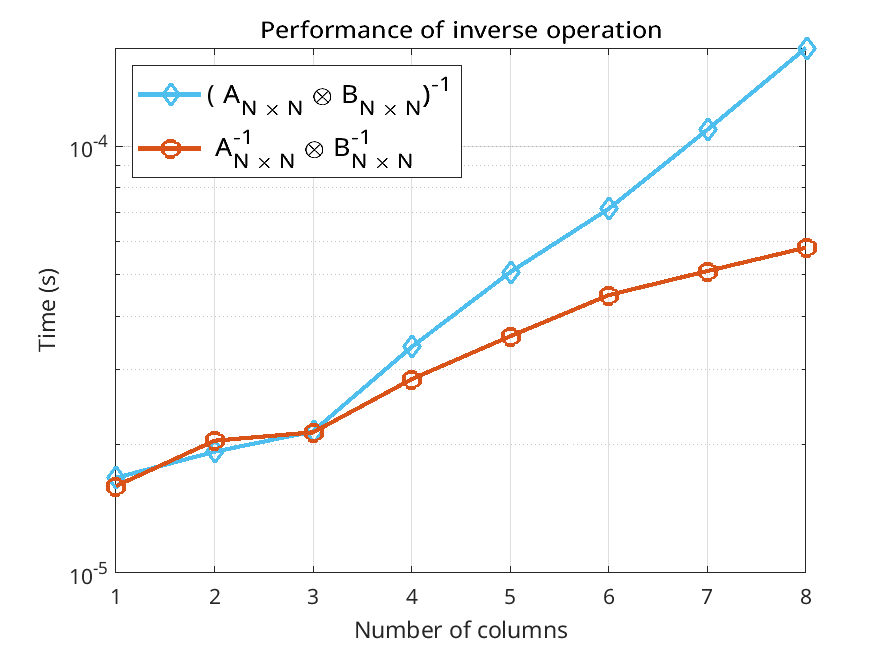
\includegraphics[width=0.75\linewidth]{figs/hw0a1.png} \par 
        \caption{Monter Carlo Experiment with 5000.}
        \label{fig:hw0a1} 
    \end{figure}

    \begin{figure}[ht!]
        \centering 
        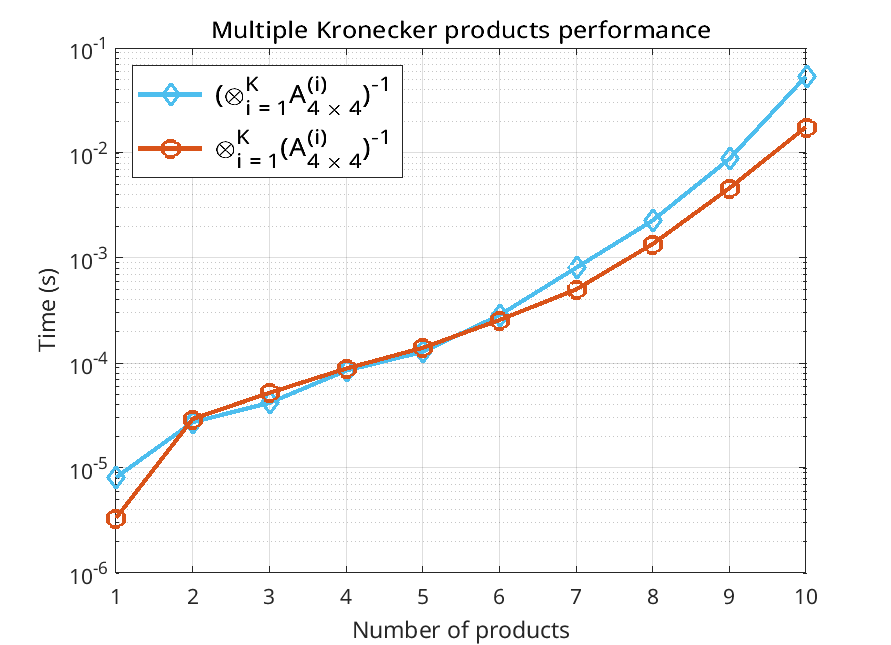
\includegraphics[width=0.75\linewidth]{figs/hw0a2.png} \par 
        \caption{Monter Carlo Experiment with 10000 runs.}
        \label{fig:hw0a2} 
    \end{figure}

    \subsection*{Show that $\text{eig}(\boldsymbol{A} \otimes \boldsymbol{B}) = \text{eig}(\boldsymbol{A}) \otimes \text{eig}(\boldsymbol{B})$}

\newpage
\section*{Homework 1 \\ Hadamard, Kronecker and Khatri-Rao Products}

    \subsection*{Run Time Perfomance of Hadamard Product}

    \begin{figure}[ht!]
        \centering 
        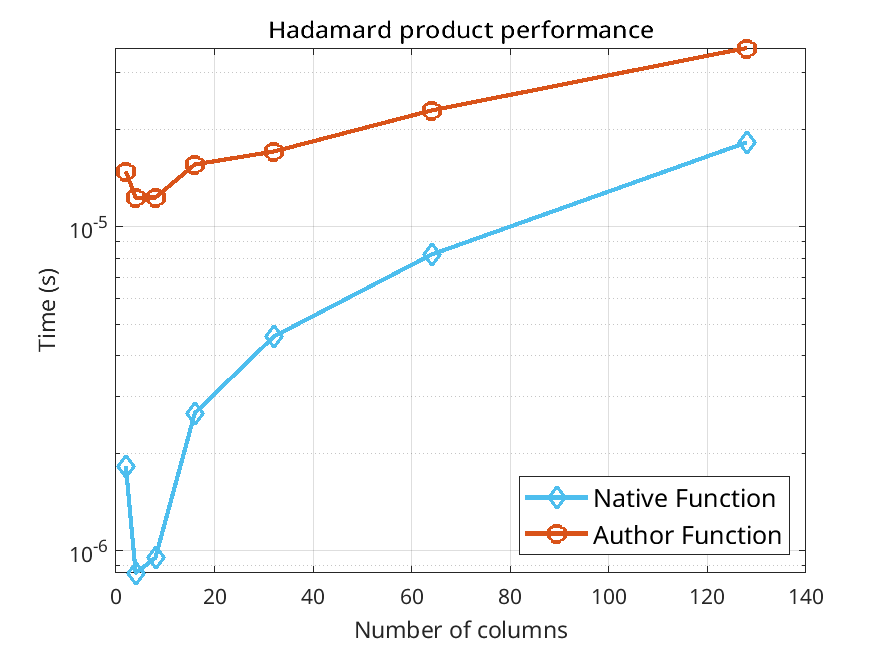
\includegraphics[width=0.75\linewidth]{figs/hw1a1.png} \par 
        \caption{Monter Carlo Experiment with 1000 runs.}
        \label{fig:hw1a1} 
    \end{figure}

    \subsection*{Run Time Perfomance of Kronecker Product}

    \begin{figure}[ht!]
        \centering 
        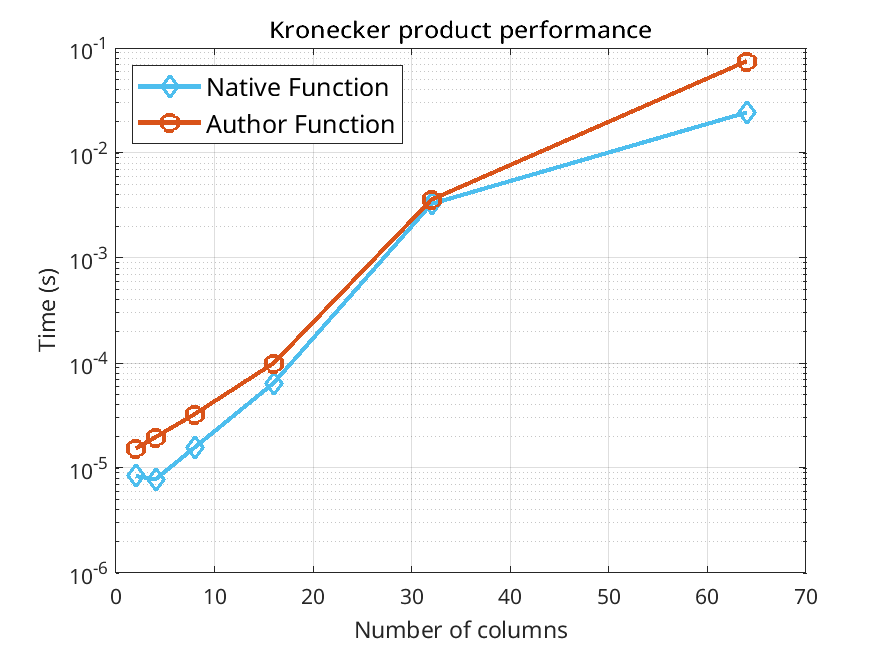
\includegraphics[width=0.75\linewidth]{figs/hw1a2.png} \par 
        \caption{Monter Carlo Experiment with 1000 runs.}
        \label{fig:hw1a2} 
    \end{figure}

    \subsection*{Run Time Perfomance of Khatri-Rao Product}

    \begin{figure}[ht!]
        \centering 
        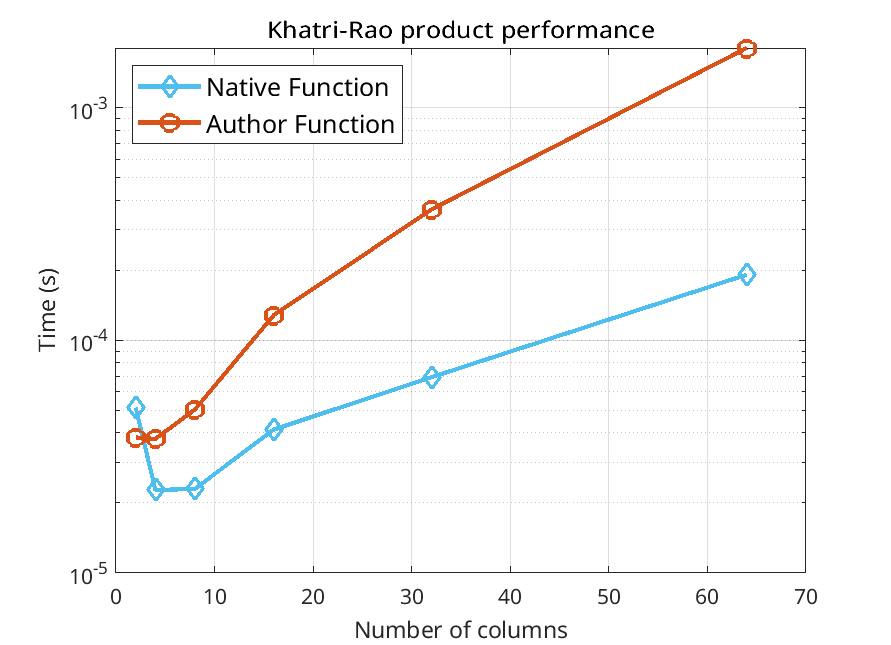
\includegraphics[width=0.75\linewidth]{figs/hw1a3.png} \par 
        \caption{Monter Carlo Experiment with 1000 runs.}
        \label{fig:hw1a3} 
    \end{figure}

\newpage
\section*{Homework 2 \\ Khatri-Rao Product Run Time}

    \subsection*{Run Time Performance of Khatri-Rao Product for Different Implementations}

    \begin{figure}[ht!]
        \centering 
        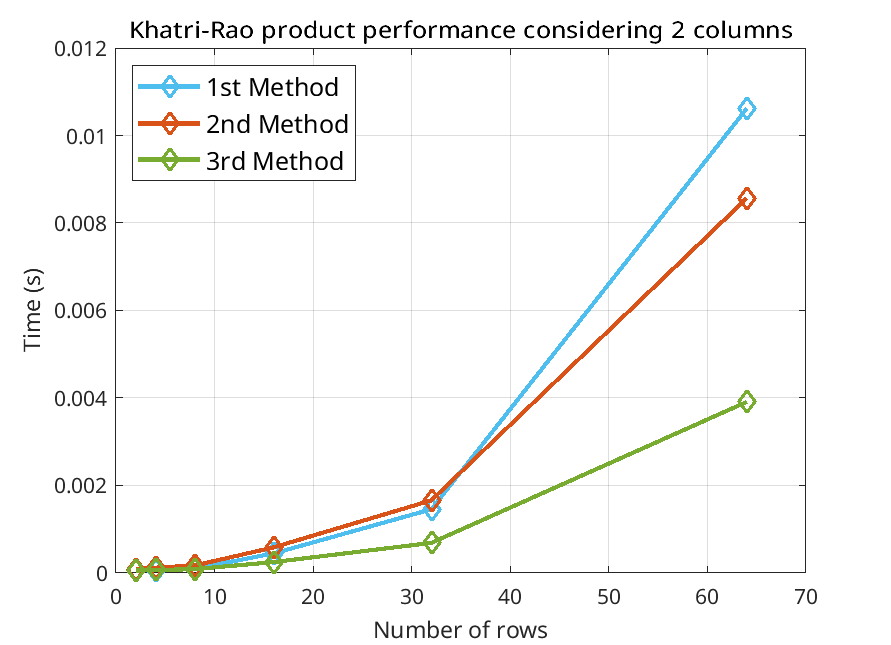
\includegraphics[width=0.75\linewidth]{figs/hw2a1.png} \par 
        \caption{Monter Carlo Experiment with 250 runs and R = 2.}
        \label{fig:hw2a1} 
    \end{figure}

    \begin{figure}[ht!]
        \centering 
        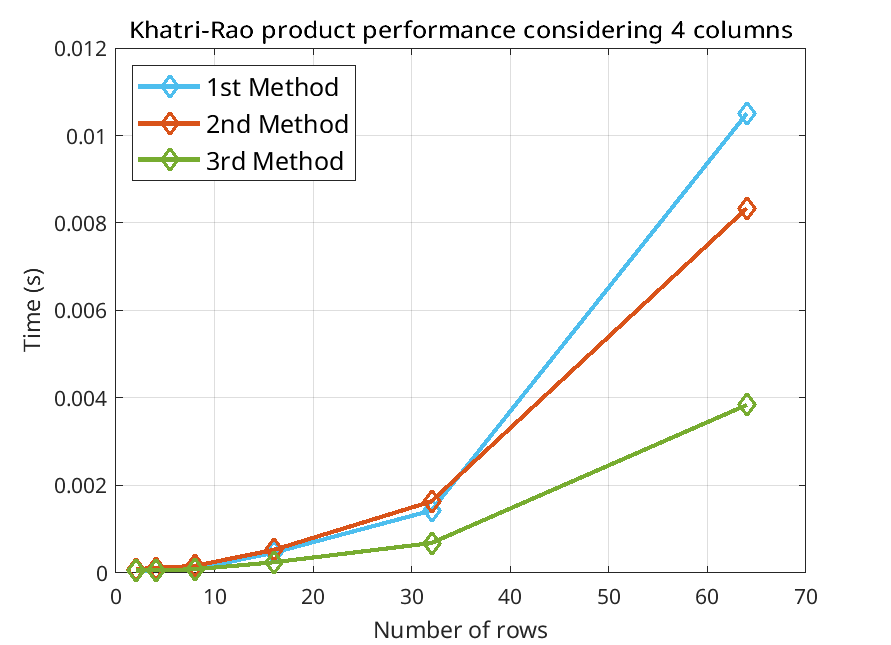
\includegraphics[width=0.75\linewidth]{figs/hw2a2.png} \par 
        \caption{Monter Carlo Experiment with 250 runs and R = 4.}
        \label{fig:hw2a2} 
    \end{figure}

    \subsection*{Run Time Perfomance of Sequential Khatri-Rao Products}

    \begin{figure}[ht!]
        \centering 
        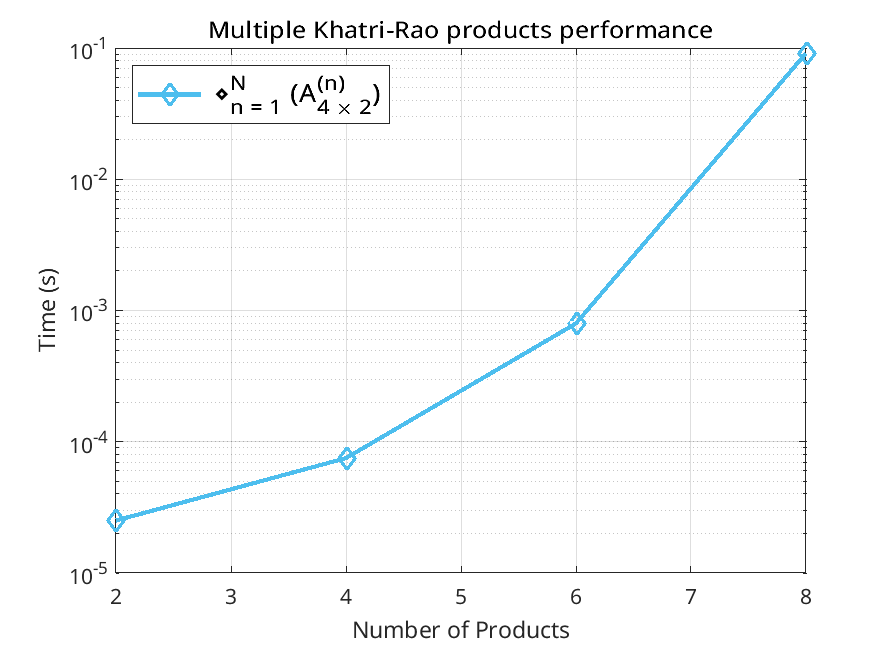
\includegraphics[width=0.75\linewidth]{figs/hw2a3.png} \par 
        \caption{Monter Carlo Experiment with 250 runs.}
        \label{fig:hw2a3} 
    \end{figure}

\newpage
\section*{Homework 3 \\ Least-Squares Khatri-Rao Factorization (LSKRF)}

    \subsection*{Implementation LSKRF}

    \subsection*{Monte Carlo Experiment}

    \begin{figure}[ht!]
        \centering 
        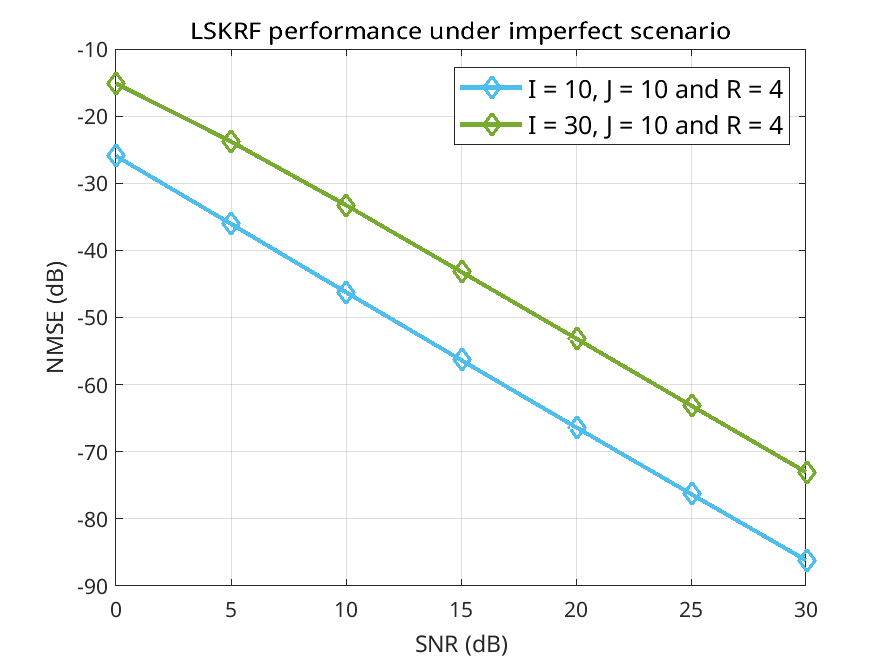
\includegraphics[width=0.75\linewidth]{figs/hw3.png} \par 
        \caption{Monter Carlo Experiment with 1000 runs for LSKRF algorithm.}
        \label{fig:hw3} 
    \end{figure}

\newpage
\section*{Homework 4 \\ Least Squares Kronecker Product Factorization (LSKronF)}

    \subsection*{Implementation LSKronF}

    \subsection*{Monte Carlo Experiment}

    \begin{figure}[ht!]
        \centering 
        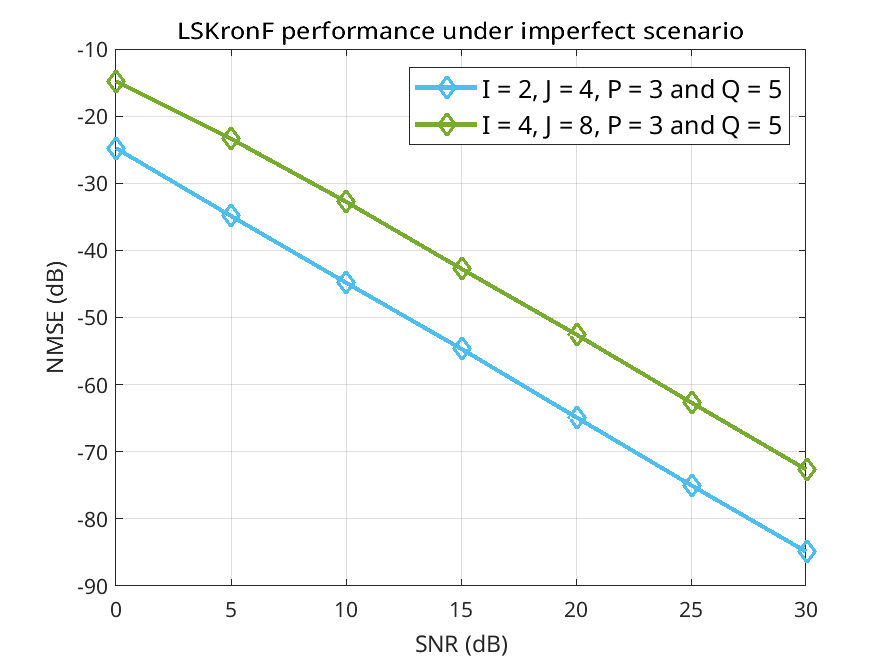
\includegraphics[width=0.75\linewidth]{figs/hw4.png} \par 
        \caption{Monter Carlo Experiment with 1000 runs for LSKronf algorithm.}
        \label{fig:hw4} 
    \end{figure}

\newpage
\section*{Homework 5 \\ Kronecker Product Singular Value Decomposition (KPSVD)}

    \subsection*{Implementation KPSVD}

    \subsection*{Validation of KPSVD}

\newpage
\section*{Homework 6 \\ Unfolding, folding, and n-mode product}

    \subsection*{Implementation unfolding, folding and n-mode product}

    \subsection*{Validation of unfolding, folding and n-mode product}

\newpage
\section*{Homework 7 \\ High Order Singular Value Decomposition (HOSVD)}

    \subsection*{Implementation HOSVD}

    \subsection*{Validation of HOSVD}

\newpage
\section*{Homework 8 \\ High Order Order Orthogonal Iteration (HOOI)}

    \subsection*{Implementation HOOI}

    \subsection*{Validation of HOOI}

\newpage
\section*{Homework 9 \\ Multidimensional Least-Squares Khatri-Rao Factorization
(MLS-KRF)}

    \subsection*{Implementation MLS-KRF}

    \subsection*{Monte Carlo Experiment}

    \begin{figure}[ht!]
        \centering 
        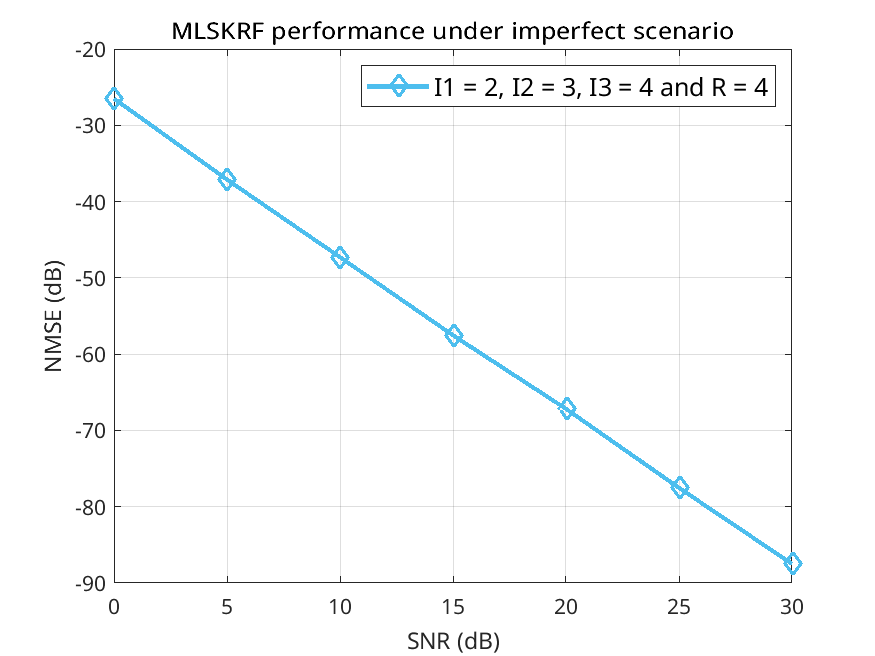
\includegraphics[width=0.75\linewidth]{figs/hw9.png} \par 
        \caption{Monter Carlo Experiment with 1000 runs for MLS-KRF algorithm.}
        \label{fig:hw9} 
    \end{figure}

\newpage
\section*{Homework 10 \\ Multidimensional Least-Squares Kronecker Factorization
(MLS-KronF)}

    \subsection*{Implementation MLS-KronF}

    \subsection*{Monte Carlo Experiment}

    \begin{figure}[ht!]
        \centering 
        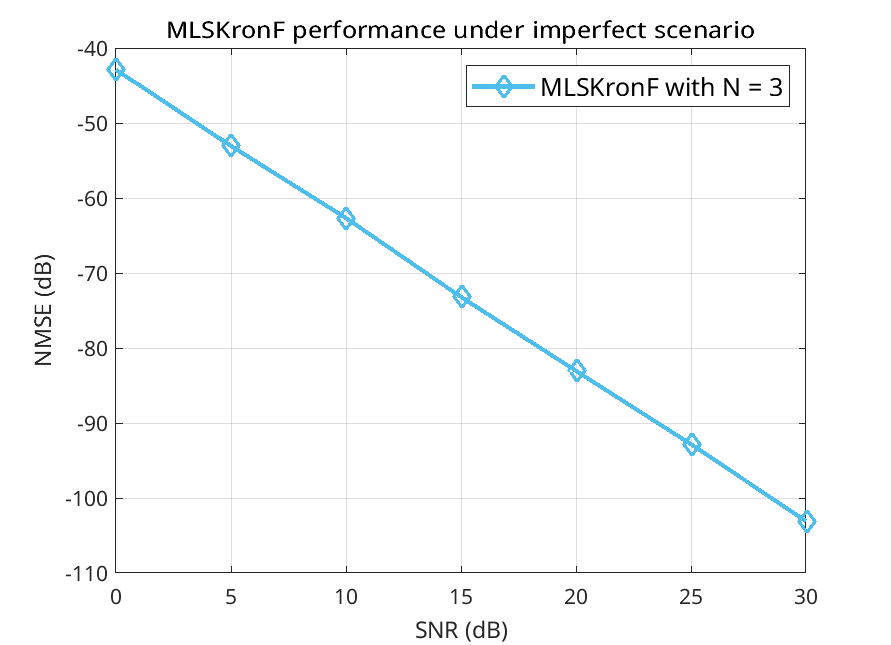
\includegraphics[width=0.75\linewidth]{figs/hw10.png} \par 
        \caption{Monter Carlo Experiment with 1000 runs for MLS-KronF algorithm.}
        \label{fig:hw10} 
    \end{figure}

\newpage
\section*{Homework 11 \\ Alternating Least Squares (ALS) Algorithm}

    \subsection*{Implementation of ALS}

    \subsection*{Monte Carlo Experiment}

    \begin{figure}[ht!]
        \centering 
        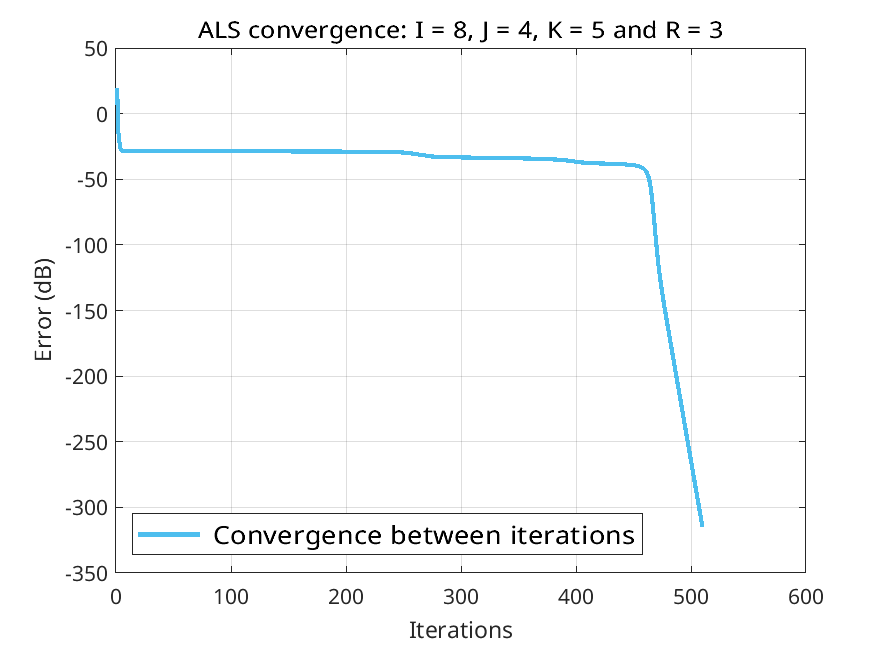
\includegraphics[width=0.75\linewidth]{figs/hw11a1.png} \par 
        \caption{Convergence behavior of ALS algorithm.}
        \label{fig:hw11a1} 
    \end{figure}

    \begin{figure}[ht!]
        \centering 
        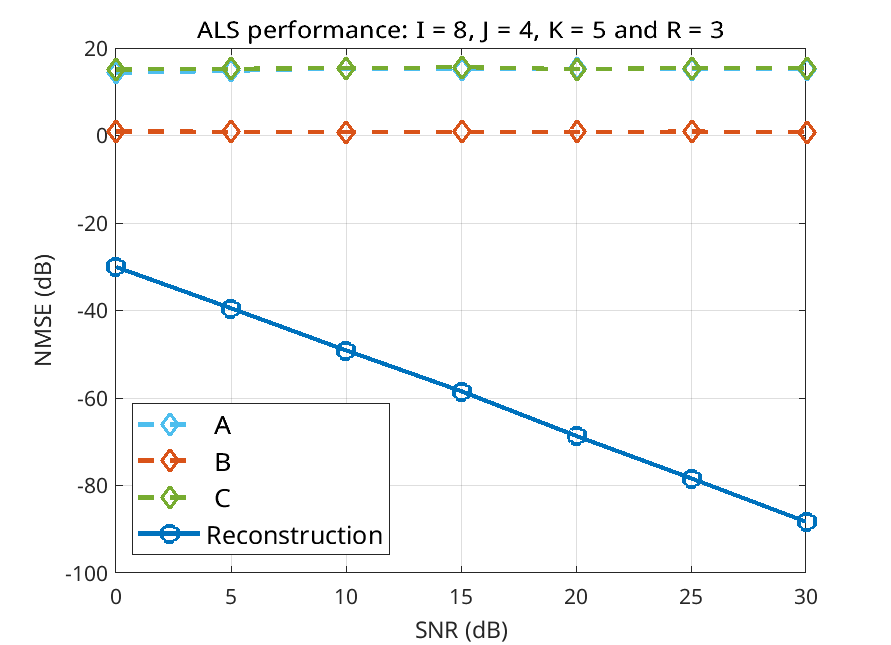
\includegraphics[width=0.75\linewidth]{figs/hw11a2.png} \par 
        \caption{Monter Carlo Experimento with 1000 runs for ALS algorithm.}
        \label{fig:hw11a2} 
    \end{figure}

\newpage
\section*{Homework 12 \\ Tensor Kronecker Product Single Value Decomposition (TKPSVD)}

    \subsection*{Implementation of TKPSVD}

    \subsection*{Monte Carlo Experiment}

    \begin{figure}[ht!]
        \centering 
        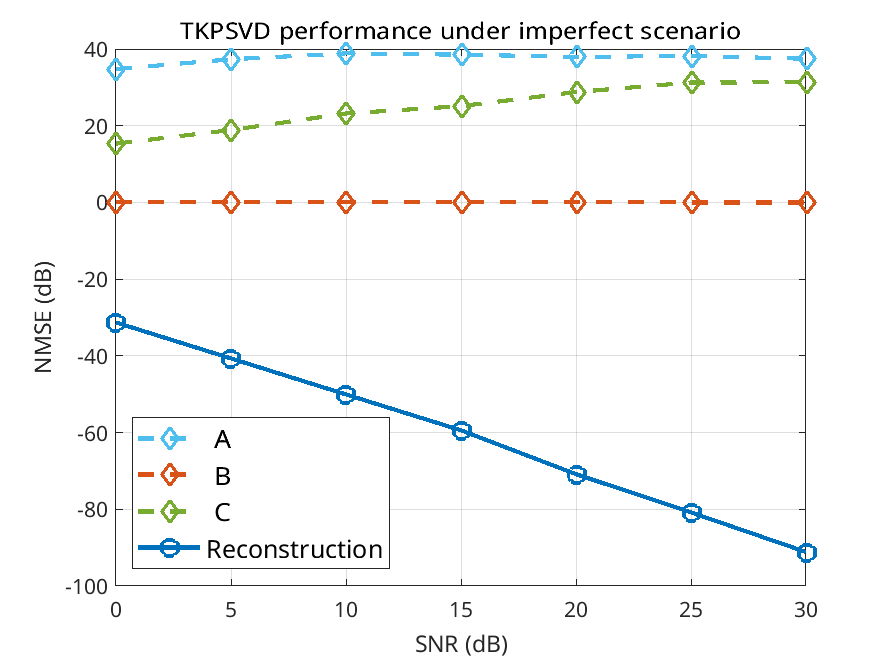
\includegraphics[width=0.75\linewidth]{figs/hw12.png} \par 
        \caption{Monter Carlo Experiment with 1000 runs for TKPSVD algorithm.}
        \label{fig:hw12} 
    \end{figure}

\newpage
\section*{Homework 13 \\ Tensor Train Single Value Decomposition (TTSVD)}

    \subsection*{Implementation of TTSVD}

    \subsection*{Monte Carlo Experiment}

    \begin{figure}[ht!]
        \centering 
        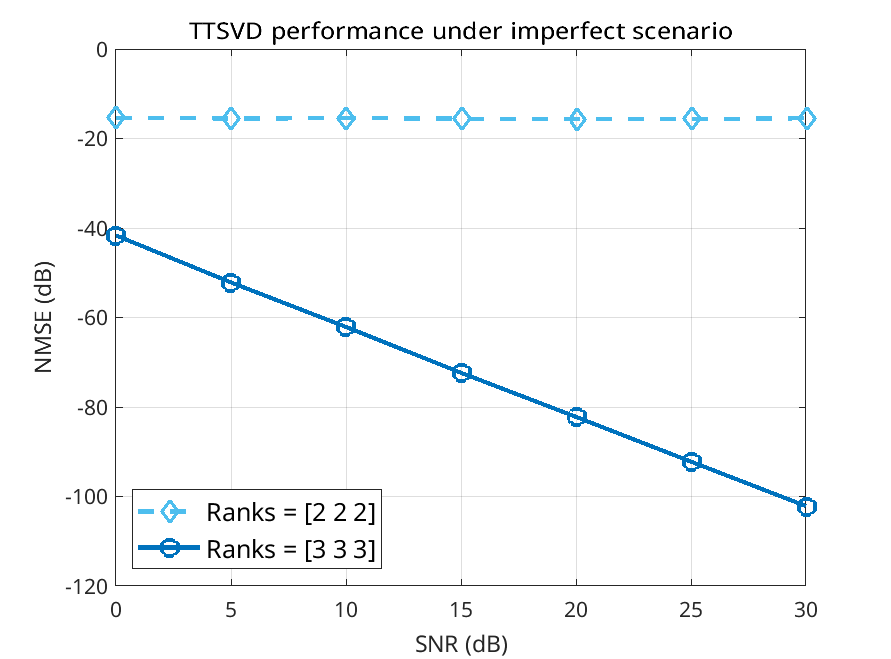
\includegraphics[width=0.75\linewidth]{figs/hw13.png} \par 
        \caption{Monter Carlo Experiment with 1000 runs for TTSVD algorithm.}
        \label{fig:hw13} 
    \end{figure}

%\bibliographystyle{ieeetr}
%\bibliography{bibliography.bib}

\end{document}

